% This file should be replaced with your file with an thesis content.
%=========================================================================
% Authors: Michal Bidlo, Bohuslav Křena, Jaroslav Dytrych, Petr Veigend and Adam Herout 2019

% For compilation piecewise (see projekt.tex), it is necessary to uncomment it and change
% \documentclass[../projekt.tex]{subfiles}
% \begin{document}

\chapter{Introduction}


%%%%%%%%%%%%%%%%%%%%%%%%%%%%%%%

\chapter{Bikefit}
This chapter explains the standard process of bikefitting, the motivation behind it and compares several commonly used software systems used for bikefitting all over the world.

\section{An introduction to bikefitting}
Cycling is massively popular activity world-wide. However, having incorrectly set position on the bike can lead to unnecessary pain and injuries. Having a position that does not suit the rider can also have a drastic effect on performance.

Due to these reasons, experts, known as bikefitters help cyclists with the setup of saddle position, handlebar position and sometimes even choosing the right parts such as saddle, handlebars or cranks.

Bikefit sessions are done mostly in person and while most professional cycling teams have a bikefitting specialist that helps to set the bikes for their athletes, they are often too costly for amateur cyclists.


This section draws from Phil Burt's Bike Fit 2nd Edition: Optimise Your Bike Position for High Performance and Injury Avoidance book \cite{burtbikefit}.

\section{Bikefit measurements}
This section describes the most common measurements used in bikefitting. These measurements can be accessed from a video using automatic bike fitting software and are simple enough to adjust by the rider themselves.

\subsection{Saddle Height}
The saddle height is a fundamental measurement that significantly impacts a rider's comfort and pedaling efficiency. It is argued to be the most important measurement in bikefitting and should be the first measurement to be adjusted \cite{burtbikefit}. Bad saddle height can even cause problems commonly associted with other measurements such as knee pain, lower back pain, neck pain, saddle sores, etc.

It is determined by considering the rider's knee angle at the bottom of the pedal stroke. Knee angle is the angle between the hip and the ankle measured at the knee joint. Burt recommends a knee angle of 35-40 degrees for average riders and even up to 30 degrees for professional cyclists \cite{burtbikefit}.

\begin{figure}[htbp]
    \centering
    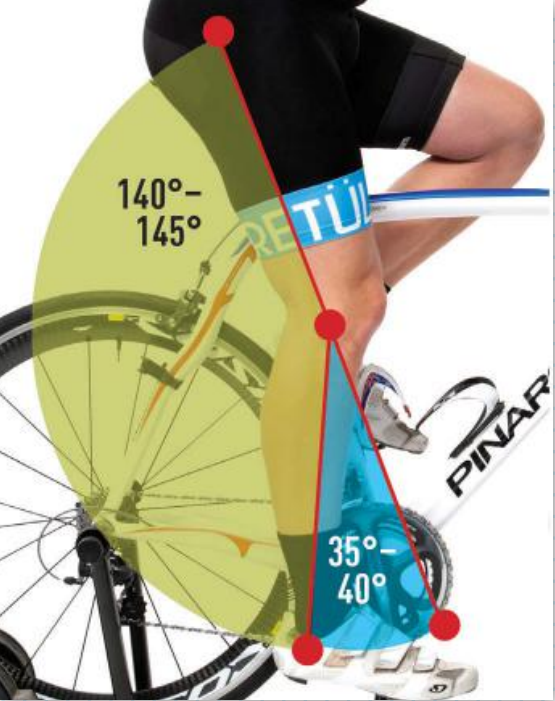
\includegraphics[width=0.5\textwidth]{obrazky-figures/burt_knee_angle.png}
    \caption{Knee extension angle of 140-145 degrees, which is often referred to as 35-40 degrees (being the angle of deviation from straight leg). Is optimal for the average rider. Taken from \cite{burtbikefit}.}
    \label{fig:saddle_height}
\end{figure}



Higher saddle height can help to better recruitment of glutens and hamstrings, which can lead to more power output. However, it requires more flexibility and can lead to injury if the rider is not flexible enough. Similarly too low saddle height can increase the compressive forces on the knee and lead to pain and injury.

Proper saddle height is therefore a balance between power output and comfort. It is also important to note that the saddle height is not the only factor that affects the knee angle. The saddle fore and aft position and the cleat position also affect the knee angle.

\subsection{Saddle Setback}
Saddle setback or saddle fore and aft position refers to the horizontal position of the saddle with respect to the bottom bracket.

\begin{figure}
    \centering
    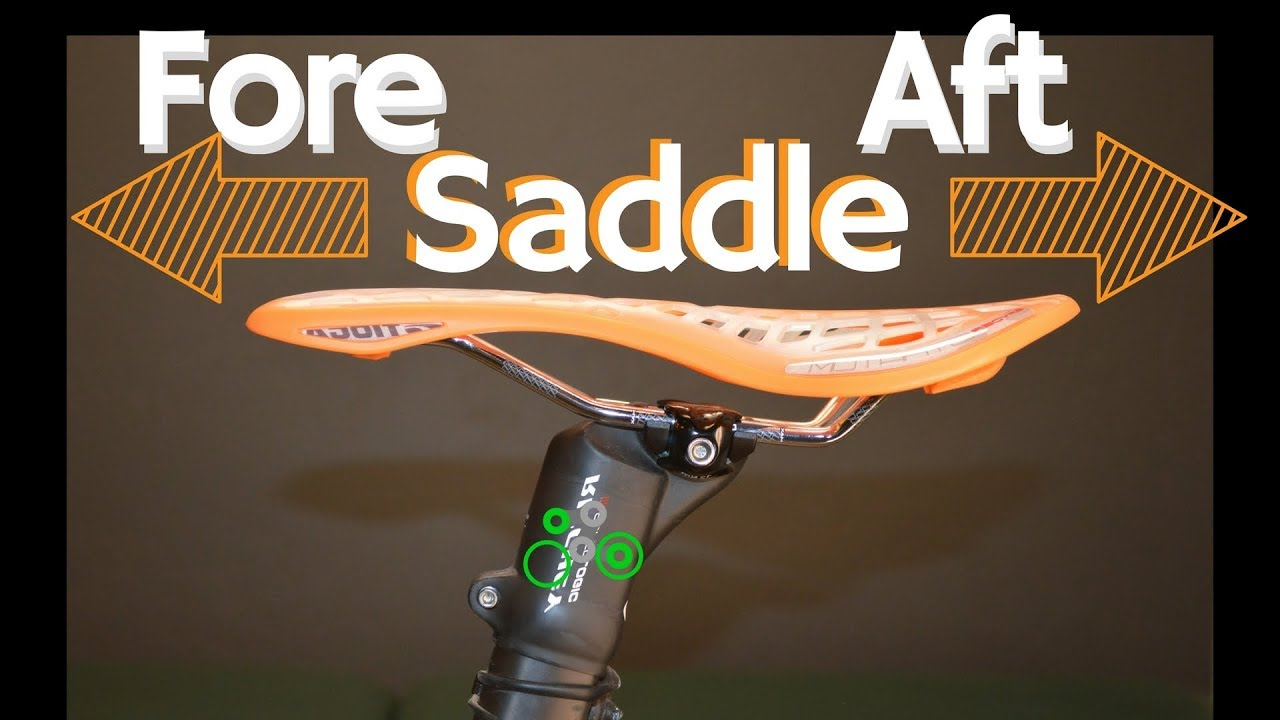
\includegraphics[width=0.8\textwidth]{obrazky-figures/saddle_fore_aft.jpg}
    \caption{Saddle setback is adjusted by sliding the saddle saddle rails forward or backward in the seatpost clamp. Taken from Bike Fit Adviser's \href{https://www.youtube.com/watch?app=desktop&v=SZhWVZq2qUc}{video} on saddle setback.}
    \label{fig:saddle_fore_aft}
\end{figure}

Setback is most often measured at the 3 o'clock position of the crank. At this position, the rider's knee should be directly above the pedal spindle. Having the knee too far back it is harder to generate power. Having the knee too far forward can lead to knee pain due to increased forces on the kneecap \cite{burtbikefit}.

Saddle setback also affects the rider's balance on the bike. Having the saddle too far forward can lead to the rider's weight being too far forward, which can lead to hand pain because of too much weight on the handlebars. Having the saddle too far back can lead to the rider's weight being too far back, which can lead to make the front wheel feel light and make the bike harder to control.

Setback also affects the rider's hip angle. Hip angle is the angle between the shoulder and the knee measured at the hip. Having the saddle more forward can lead to a more open hip angle, which can lead to more power output and more space between the rider's torso and legs at the top of the pedal stroke. This is why time trial bikes have a more forward saddle position.



\subsection{Handlebar Height and Reach}
Handlebar height measures how high the handlebars are in relation to the saddle. Handlebar reach measures how far the handlebars are in relation to the saddle.

Handlebar height influences mainly torso angle and to and also shoulder angle. Torso angle is the angle between the shoulder and the level plane measured at the hip. It is also known as the back angle. Shoulder angle is the angle between the hip and wrist measured at the shoulder. Handlebar reach influences mainly shoulder angle.

Handlebar height can be adjusted by changing the number of spacers under the stem or by changing the stem itself. Handlebar reach can be adjusted by changing the stem length or by changing the handlebars themselves.

While optimal handlebar height and reach are highly individual, there are some general guidelines. For example, a more upright position is more comfortable and is therefore recommended for longer rides. A more aggressive position is more aerodynamic and is therefore recommended for racing. Burt recommends back angle of about 45 degrees for average riders and shoulder angle of about 90 degrees with the elbow slightly bent \cite{burtbikefit}. For faster riders, the back angle can be lowered up to 30 degrees with more open shoulder angle. For more upright riders, the back angle can be increased up to 55 degrees with more closed shoulder angle.


%%%%%%%%%%%%%%%%%%%%%%%%

\section{Existing software systems for bikefitting}

\subsection{MyVeloFit}
\href{https://www.myvelofit.com/}{MyVeloFit}  is a web application that uses pose estimation model to predict the joint locations for a side view video of the user pedaling their bike on an indoor trainer. Based on location of these joints, joint angles are then computed. On the basis of these angles and their relation to average angles, suggestions are made for adjusting the position of the saddle and handlebars.

The fitting process starts with the rider filling out questionaire about their mobility. This is then used to adjust the recommended angle ranges. For example: if the user has lower shoulder mobility, recommended ranges for shoulder angle will be increased so the user is not stretched forward so much.

After creating the user profile, user can create a fit session for one specific bike. In the process, the user selects their fit goal (performance, comfort, or balanced) and the type of bike they are using (road, gravel, mtb, triathlon, hybrid, or stationary). This also changes the recommended angle ranges.

\subsubsection{Predicted keypoints}
MyVeloFit predicts 6 joint locations for the camera facing side of the body. Most common pose estimation models predict similar keypoints. However, keypoints commonly used to adjust the position of the saddle, such as the heel and the fifth metatarsal of the foot, are missing.


\begin{itemize}
    \item Ankle
    \item Knee
    \item Hip
    \item Shoulder
    \item Elbow
    \item Wrist
\end{itemize}

\begin{figure}[htbp]
    \centering
    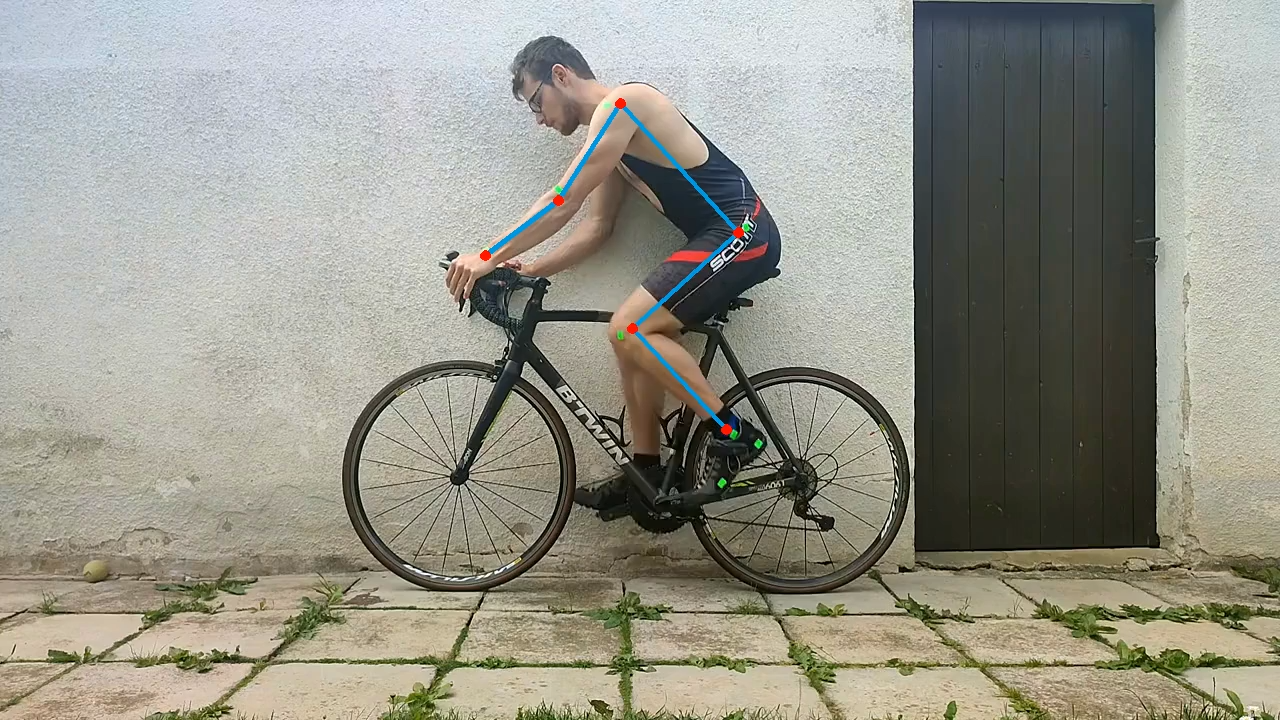
\includegraphics[width=\textwidth]{obrazky-figures/myvelofit_keypoints.png}
    \caption{Side view image with predicted keypoints in MyVeloFit.}
    \label{fig:myvelofit_keypoints}
\end{figure}

From the joint angles for every frame, some are selected for computing the joint angles at the top of the pedal stroke, front of the pedal stroke and bottom. Every position uses different angle ranges and even which angles are taken into account.

\begin{figure}[htbp]
    \centering
    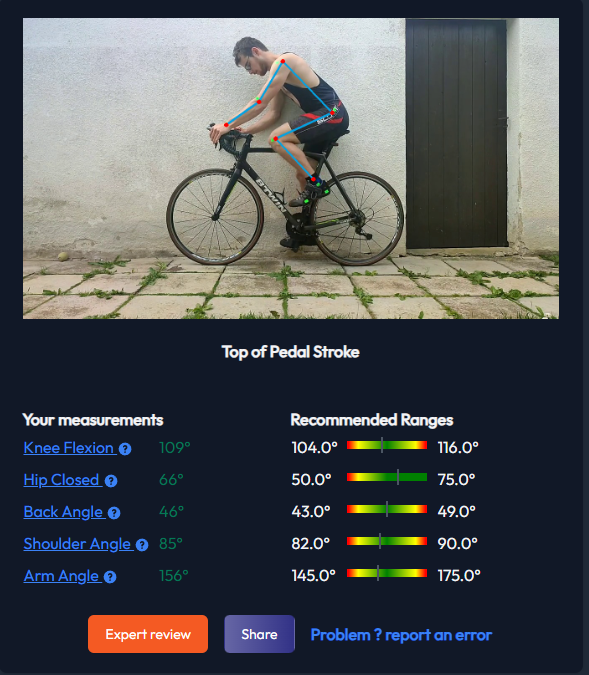
\includegraphics[width=0.6\textwidth]{obrazky-figures/myvelofit_top.png}
    \caption{Predicted joint angles at the top of the pedal stroke in MyVeloFit.}
    \label{fig:myvelofit_top}
\end{figure}

Based on the angles computed for parts of the pedal stroke, MyVeloFit then makes suggestions for saddle height, saddle fore and aft, handlebar height and handlebar reach.

\begin{figure}[htbp]
    \centering
    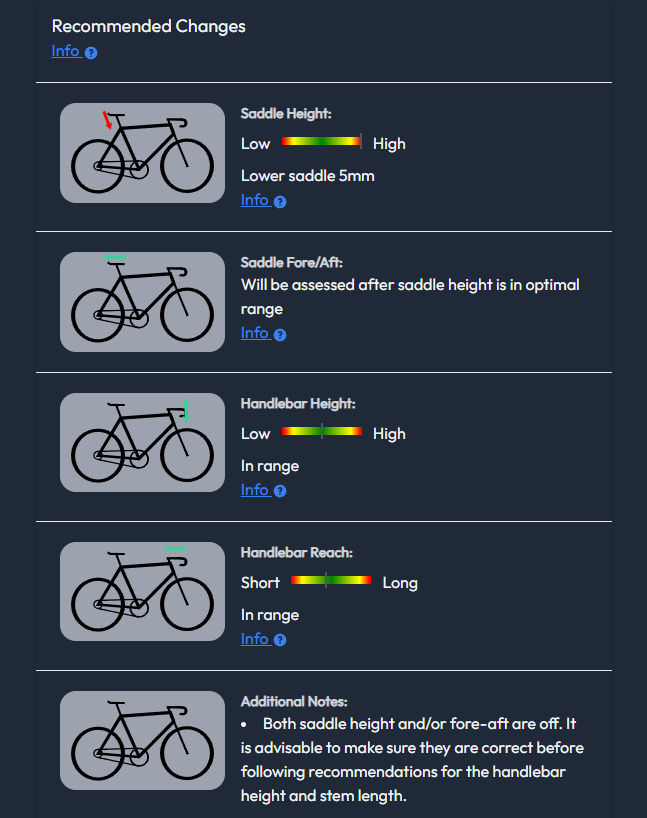
\includegraphics[width=0.6\textwidth]{obrazky-figures/myvelofit_suggestions.png}
    \caption{Recommended changes to the bike position based on the angles computed by MyVeloFit.}
    \label{fig:myvelofit_suggestions}
\end{figure}

Overall, MyVeloFit is relatively easy to use and its joint predictions are fairly accurate. However, it has few disadvantages:

\begin{itemize}
    \item Only the most basic keypoints are used.
    \item Every video is converted to 30 FPS and cut down to 10 seconds.
    \item Video processing and keypoint predictions are slow (3-5 minutes).
    \item Requires subscription to get joint angles and recommended changes. Either a one time payment of 35 US dollars for access for 1 person and 1 bike for 2 weeks or 75 US dollars annually for unlimited number of bikes and people.
\end{itemize}


\subsection{Retül}
\href{https://www.retul.com/}{Retül} is a bike fitting system employing 3D motion capture technologys. It utilizes infrared LED markers placed on specific body points to track the rider's movements dynamically while cycling. The led markers are tracked by multiple infrared cameras placed around the rider. The cameras surprisingly capture only 18 frames per second. Despite this research \cite{retulReliability} shows that the system is relatively reliable compared to 3d motion capture systems with higher frame rates.

Retül uses 8 markers placed on both sides of the rider's body. These markers are placed on the following locations:

\begin{itemize}
    \item Fifth metatarsal of the foot
    \item Heel
    \item Ankle
    \item Knee
    \item Hip
    \item Shoulder
    \item Elbow
    \item Wrist
\end{itemize}

The markers are placed by the fitter on the rider's body. Accurate placement of the markers is crucial for the system to work properly. Even small deviations can lead to inaccurate results.

\begin{figure}[htbp]
    \centering
    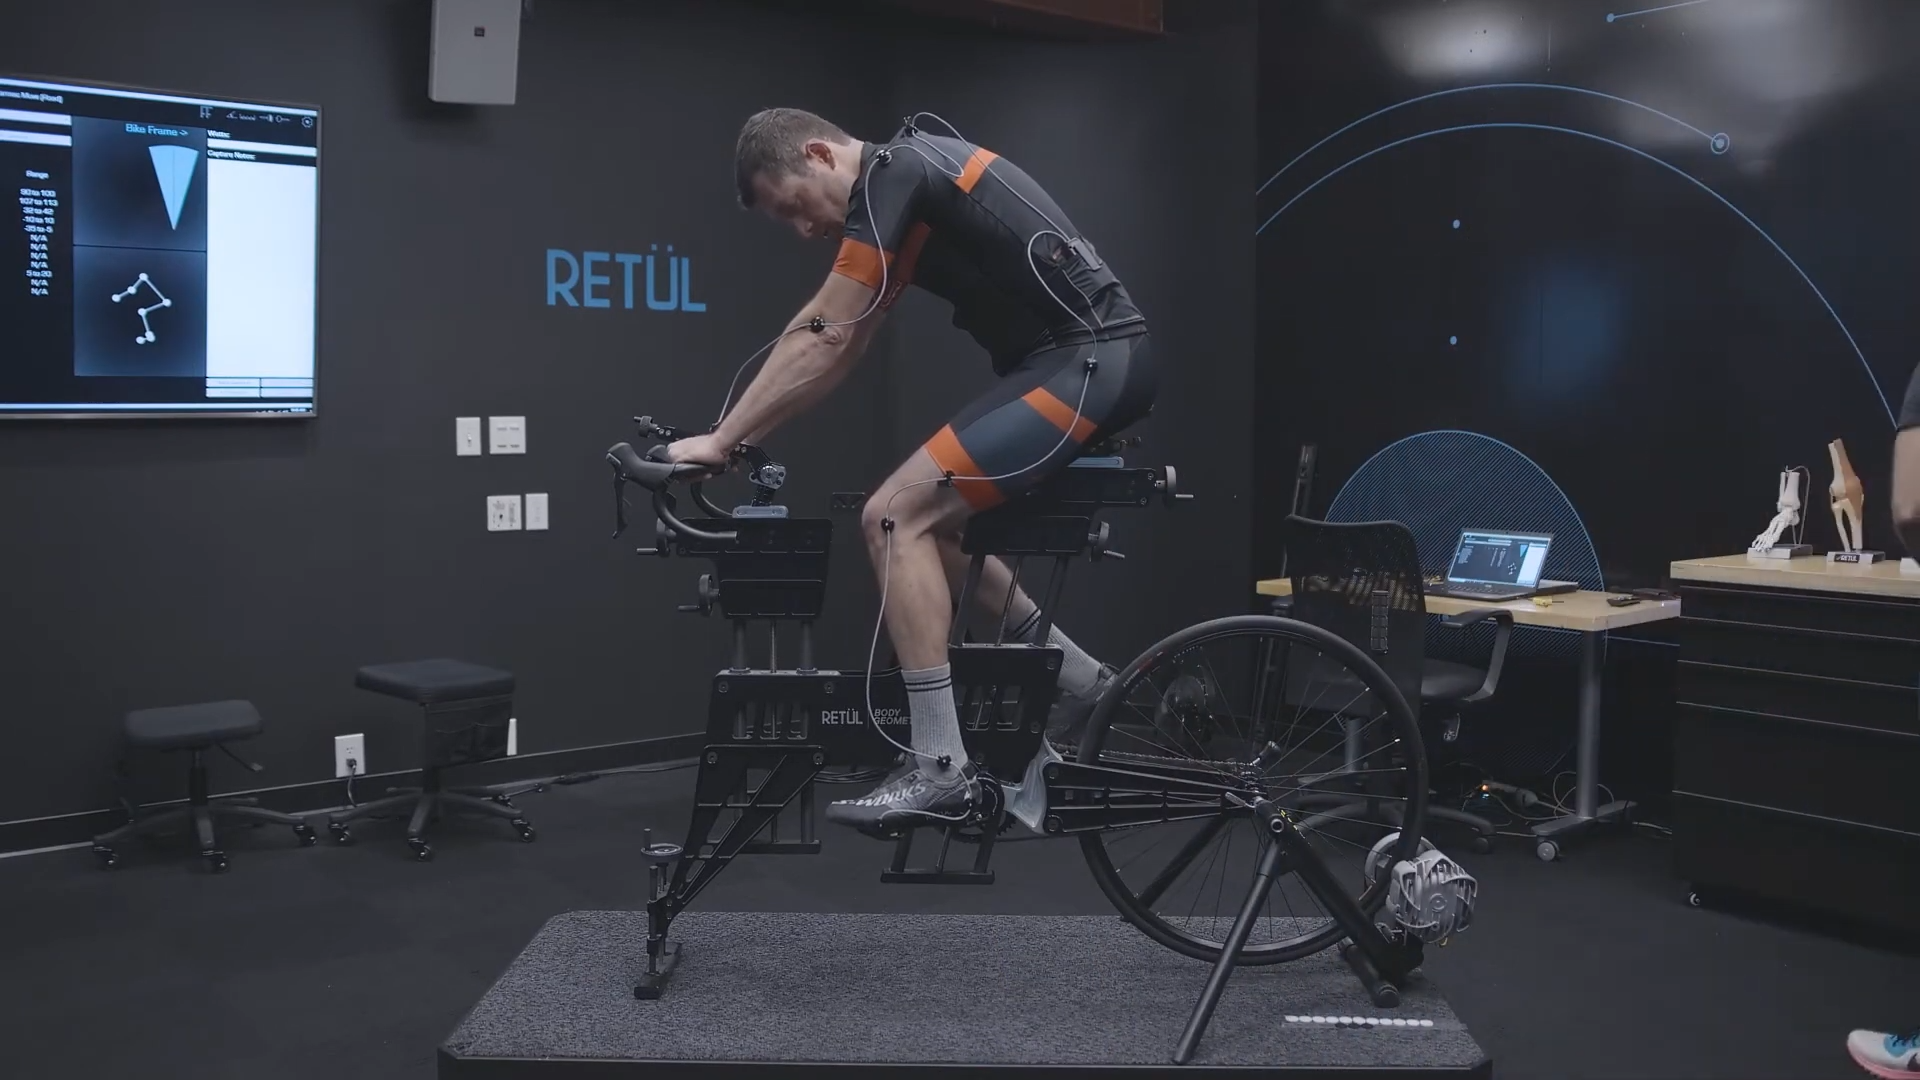
\includegraphics[width=\textwidth]{obrazky-figures/retul_markers.png}
    \caption{Placement of the markers used by Retül. (Screenshot from instructional instructional video by Retül \cite{retulMarkersYoutube}.)}
    \label{fig:retul_markers}
\end{figure}

Retül's fitting process involves setting up the bike on a trainer equipped with the system. During the session, the rider performs various motions and pedal strokes while the Retül system captures real-time data on joint angles and movements.

Data Captured by Retül includes a wide range of joint angles and movements such as knee angles at top of the pedal stroke and bottom of the pedal stroke, hip angles throughout the pedal stroke, shoulder, elbow, and wrist positions in relation to handlebar reach and drop, as well as ankle and foot movement concerning cleat positioning and alignment.

\begin{figure}[htbp]
    \centering
    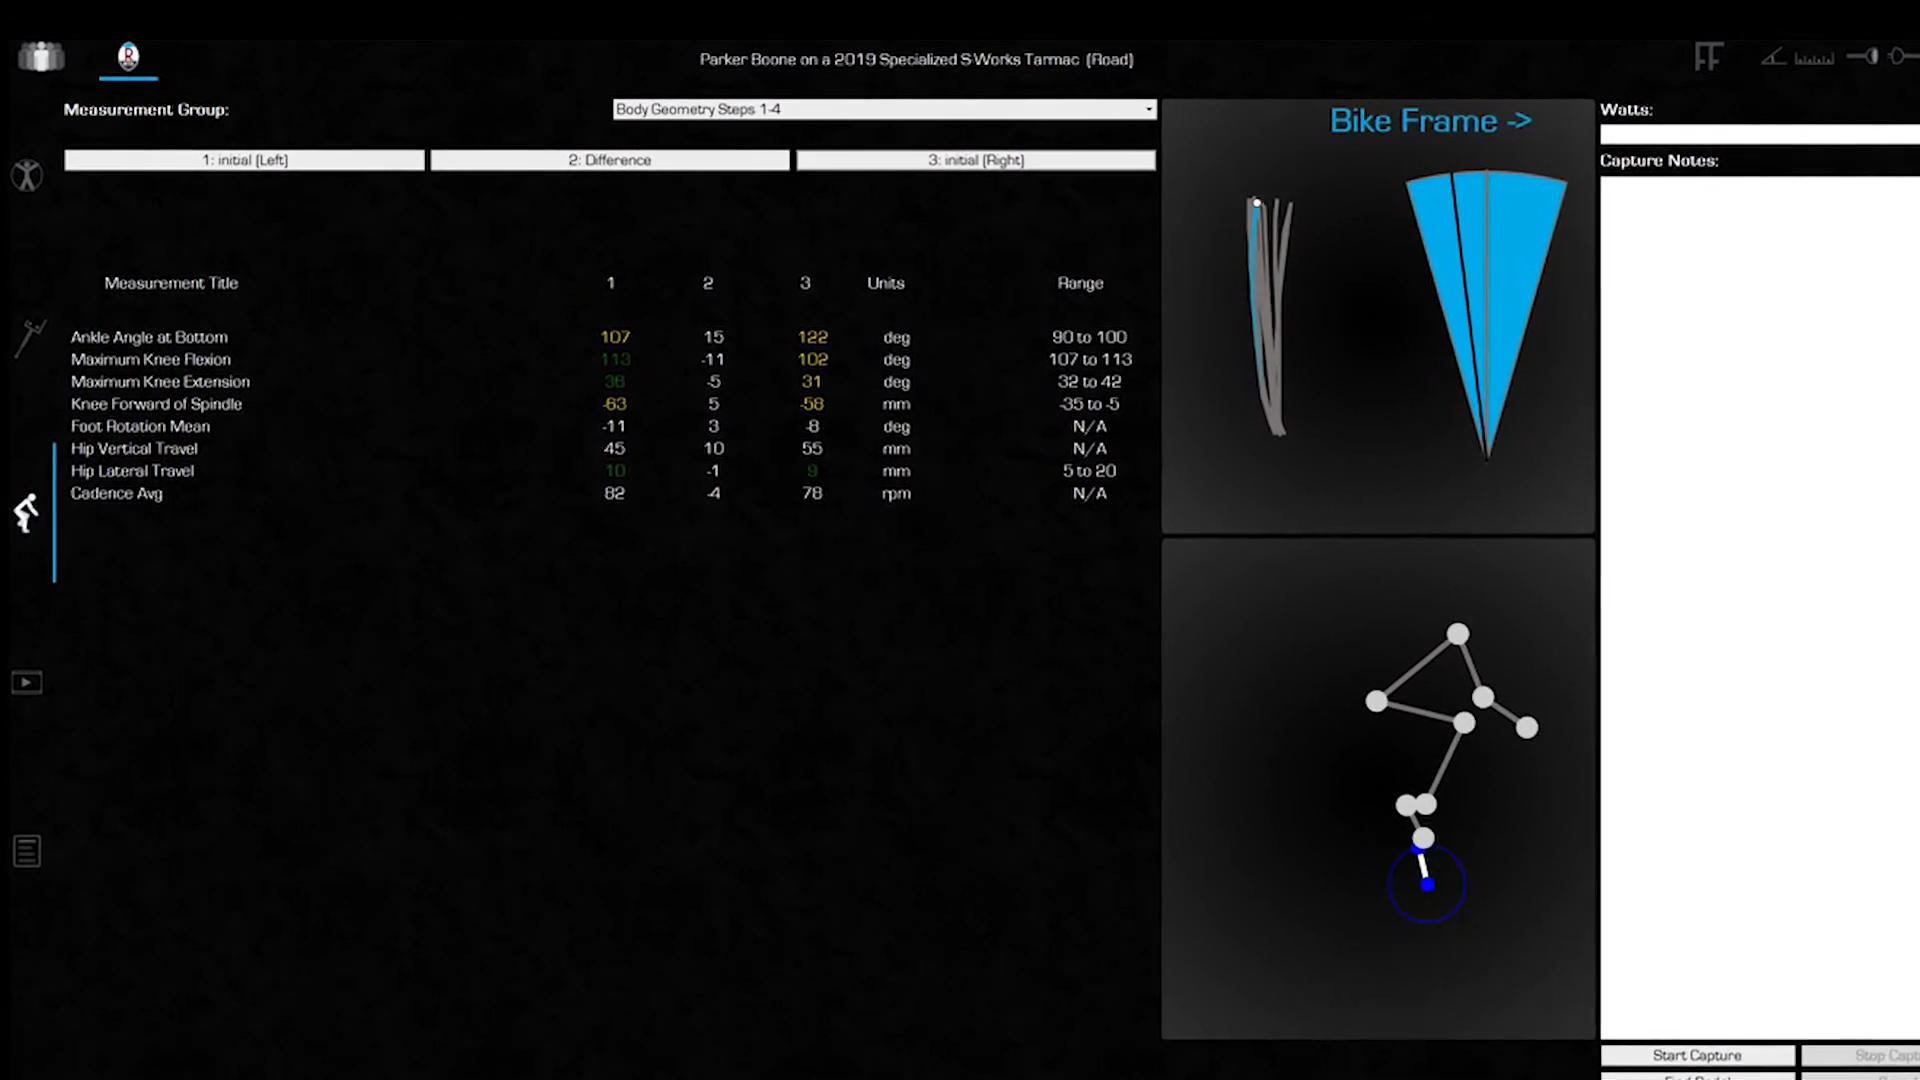
\includegraphics[width=\textwidth]{obrazky-figures/retul_app.png}
    \caption{Retül's software showing the captured data. (Screenshot from  instructional video by Retül \cite{retulScreenYoutube}.)}
    \label{fig:retul_app}
\end{figure}

The normal ranges for these angles were constructed based on the data collected from thousands cyclists. However, these cyclists were not necessarily optimally fitted to their bikes. Therefore, the normal ranges may not be based on the optimal position for the rider.

Based on the captured data, Retül compares the rider's position to the normal ranges. Based on this comparison, the fitter can make changes to the bike position.

Despite the fact that Retül is a very popular bike fitting system, it has some important disadvantages:
\begin{itemize}
    \item Costly equipment and setup requirements, limiting accessibility to some individuals or smaller bike shops.
    \item The need for trained Retül bike fitters to interpret and implement fitting recommendations effectively.
    \item Requires in-person fitting sessions. These sessions can be time-consuming and costly.
\end{itemize}


\subsection{BikeFast Fit Elite}
\href{https://www.bikefastfit.com/}{BikeFast Fit Elite} is an iOS and Mac OS application that uses pose estimation model to predict the joint locations for a side view video of the user pedaling their bike on an indoor trainer. Compared to MyVeloFit, it uses additional keypoints for the fifth metatarsal of the foot and the heel.

\begin{figure}[htbp]
    \centering
    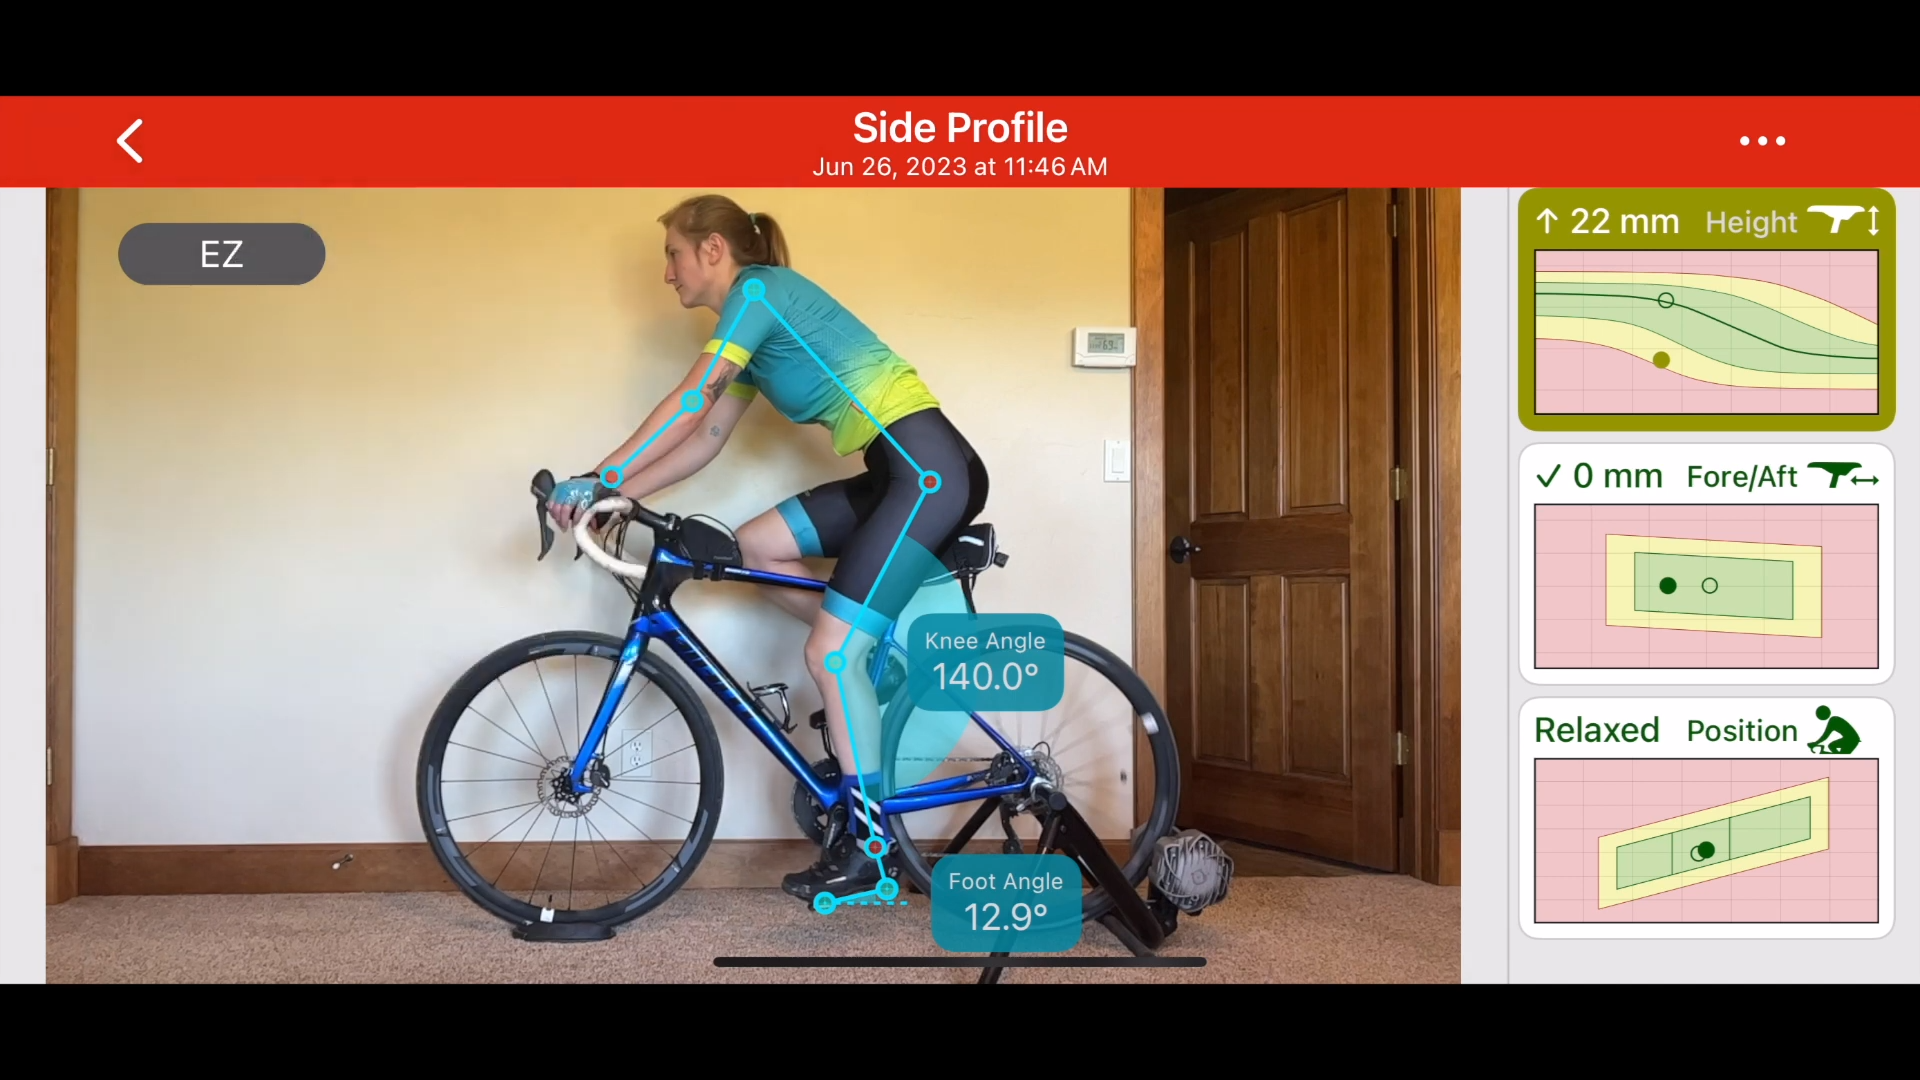
\includegraphics[width=\textwidth]{obrazky-figures/bike_fast_fit_elite.png}
    \caption{Side view image with predicted keypoints in BikeFast Fit Elite. (Screenshot from promotional video \cite{bikeFastFitElitev2Youtube} by BikeFast Fit Elite.)}
    \label{fig:bikefastfit_keypoints}
\end{figure}

Similarly to MyVeloFit, it suggest changes to the saddle height and fore and aft position but it does not suggest changes to the handlebar position, arguing that the handlebar position is based on individual goals and flexibility.

Additionally, it also provides front view knee tracking to address possible knee wobble and asymmetry.

The app costs 19.99 US dollars and does not require a subscription. However, it is only available for iOS and Mac OS. Also it only captures 3.5 seconds of video.


\subsection{Kinovea}


\subsection{Posiclist}



%%%%%%%%%%%%%%%%%%%%%%%%%%%%%%%%%%%%%

\chapter{Pose estimation algorithms}

\section{RTMPose}

\section{HRNet}

\section{YOLOX}

\section{VIP-NAS}

\section{Evaluation}
The goal of this section is to evaluate the performance of pose estimation models on the task of side view pose estimation of cyclists and find the best model for use in the bikefit application.

The models are evaluated on a custom dataset, which is described in section \ref{evaluation_dataset}. The evaluation metrics are described in section \ref{evaluation_metrics}. The results are shown in section \ref{evaluation_results}.

The models are ran using the MMPose framework \cite{mmpose2020}, with the Inferencer API and the PyTorch backend. Topdown models (models that require inputs cropped to the bounding box of the person) use the RTMDet-nano model \cite{rtmdet} from the MMDetetection framework \cite{mmdetection} for person detection.

Since no models predict the fifth metatarsal of the foot, the small toe landmark is used instead for the models that predict it.



\subsection{Evaluation dataset}
\label{evaluation_dataset}
To accurately measure the performance of a pose estimation model, it is necessary to have a dataset with ground truth annotations. Since there is no such dataset for side view pose estimation of cyclists, new small evaluation dataset was created. It consists of 12 videos in 3 different enviroments with various camera angles and riding positions (riding on hoods, drops, tops and aero position on the drops). The videos were shot in FullHD resolution at 30 FPS.

Before shooting the videos, orange colored markers were placed on the camera-facing side of the rider's body. These markers were placed on the following locations:

\begin{itemize}
    \item Fifth metatarsal of the foot
    \item Heel
    \item Ankle
    \item Knee
    \item Hip
    \item Shoulder
    \item Elbow
    \item Wrist
\end{itemize}

\begin{figure}[htbp]

    \centering
    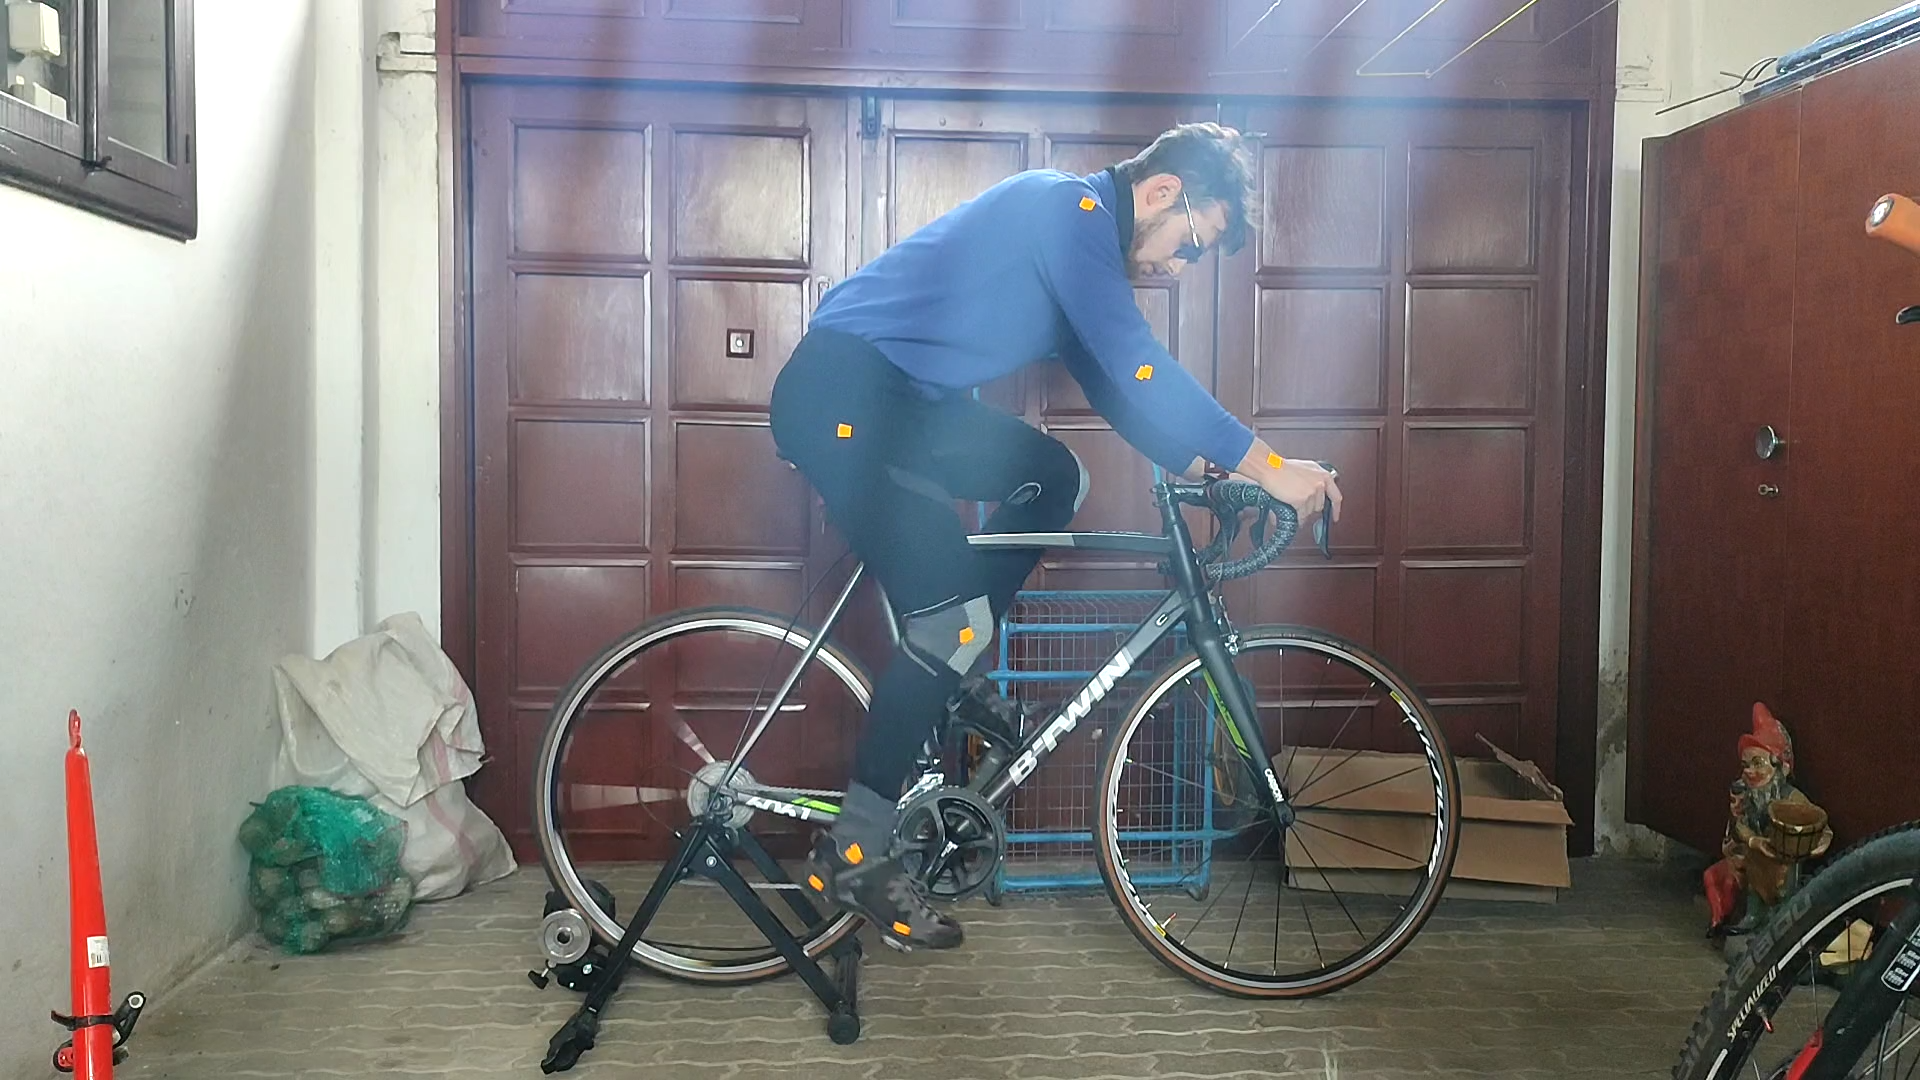
\includegraphics[width=1\linewidth]{obrazky-figures/eval_dataset_in_hoods.png}

    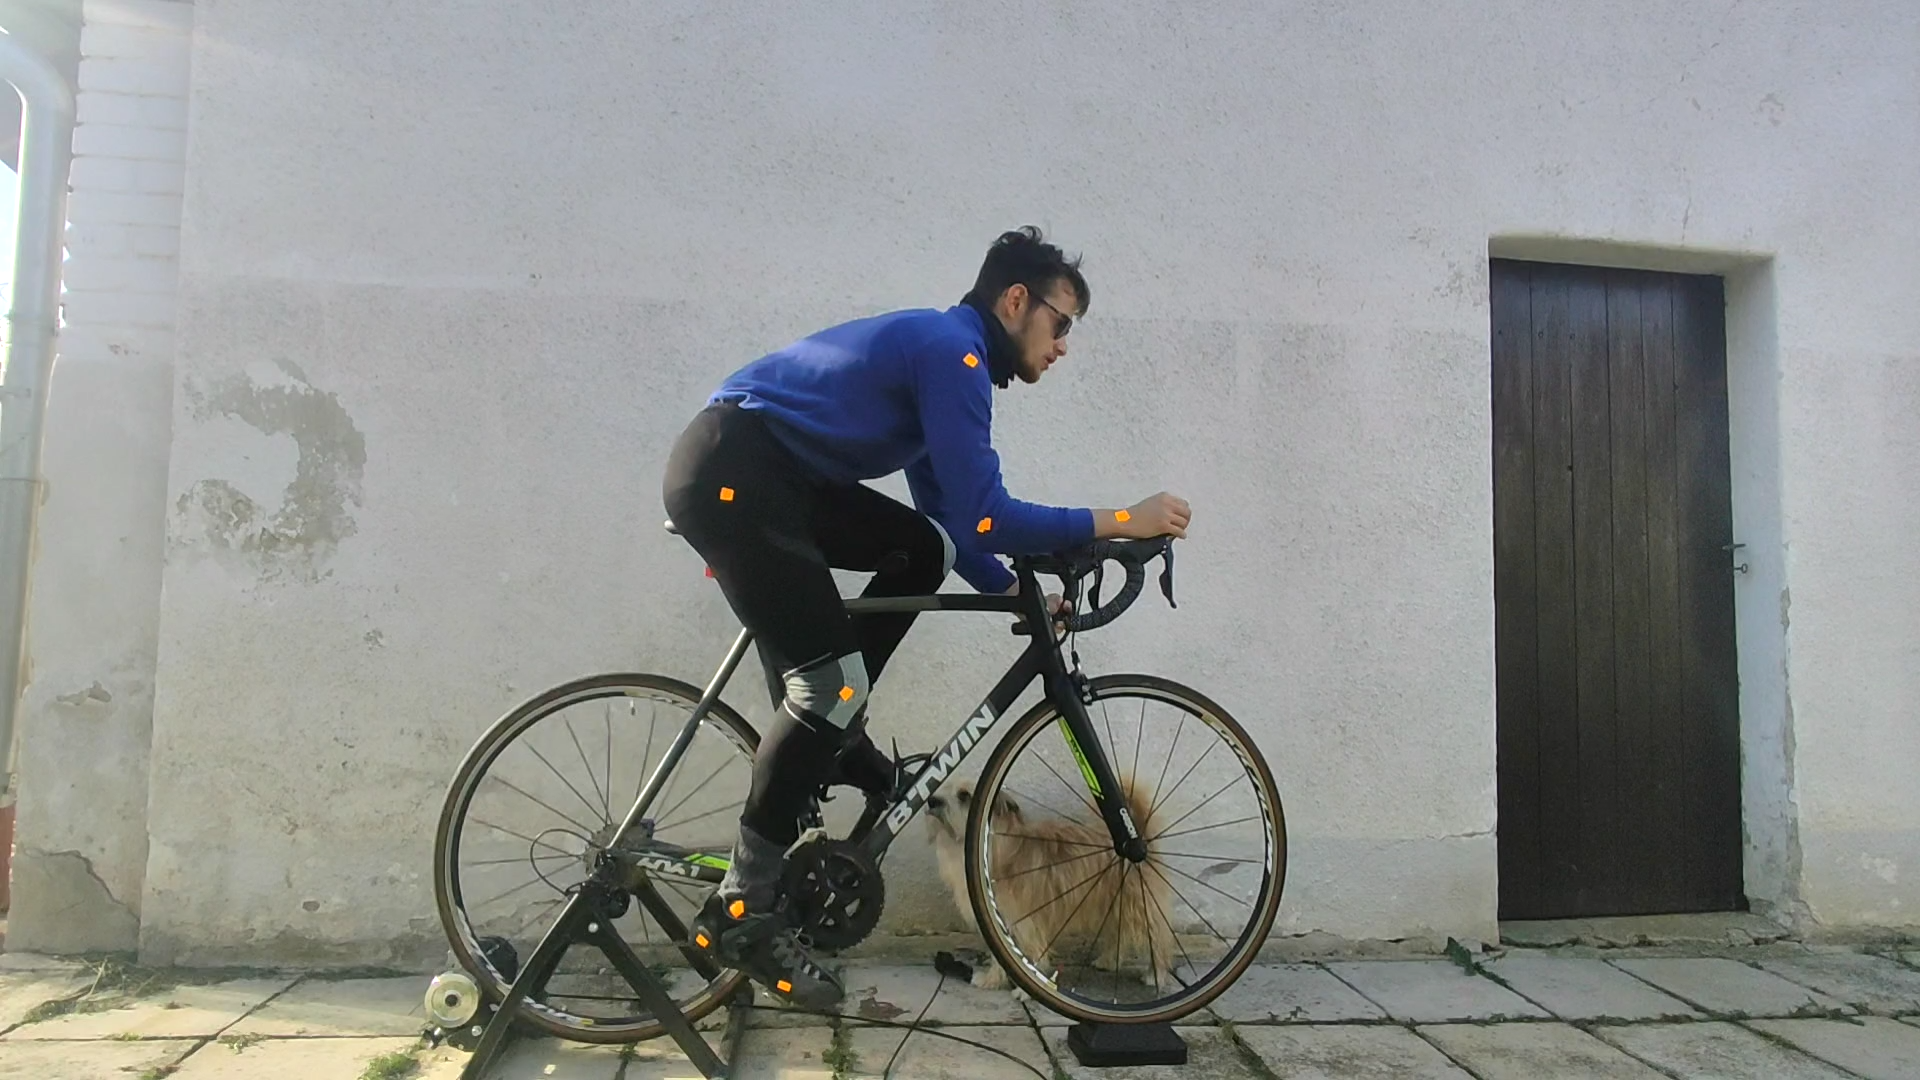
\includegraphics[width=1\linewidth]{obrazky-figures/eval_dataset_out_aero.png}

    \caption{Examples of the evaluation dataset. The first video shows the rider pedaling indoors on the hoods. The second video shows the rider pedaling outdoors in the aero position on the hoods. The orange stickers are used as ground truth annotations.}


    \label{fig:evaluation_markers}
\end{figure}

To annotate the videos, the markers were tracked using the first version of the bikefit application described in \textcolor{red}{TODO}. The application tracks the markers in a lower resolution. To get the ground truth annotations, the marker positions were then scaled to the original resolution of the video.

\subsection{Evaluation Metrics}
\label{evaluation_metrics}

In assessing the performance of pose estimation models, widely used metrics, such as Mean Average Precision (mAP), or Object Keypoint Similarity (OKS) may not adequately gauge accuracy in scenarios involving video data where all keypoints of interest are consistently visible and accurately predicted. Similarly, relying solely on the L2 distance for evaluation proves inadequate due to the inherent variations in scale among different videos.

As an alternative approach, a novel metric called \textbf{Bounding Box Normalized Distance (BBND)} has been employed. This metric involves calculating the ratio of the Euclidean distance to the average dimension of the bounding box, scaled by a factor of 100, so it can be expressed as a percentage:

$$ \text{BBND} = \frac{\text{dist}}{\frac{\text{bbox.w} + \text{bbox.h}}{2}} \times 100 $$

Here, in the BBND formula:
\begin{description}
    \item[$\text{BBND}$:] Bounding Box Normalized Distance, which is the evaluation metric being proposed.
    \item[$\text{dist}$:] Euclidean distance between the predicted keypoints and the ground truth keypoints.
    \item[$\text{bbox.w}$:] Width of the bounding box encompassing the keypoints.
    \item[$\text{bbox.h}$:] Height of the bounding box encompassing the keypoints.
\end{description}

This adjustment allows for a scaled representation of the distance metric, effectively normalizing it with respect to the average bounding box dimension. BBND offers easy to interpret results, with a lower value indicating a more accurate prediction. It also allows for a more direct comparison of the performance of different models, as the metric is not affected by the scale of the video.

\subsection{Results}
\label{evaluation_results}
At first the models are evaluated using only the keypoints that all models predict. These keypoints are the ankle, knee, hip, shoulder, elbow and wrist. The results are shown in table \ref{tab:evaluation_results_coco}. The best results are achieved by the rtmpose-l-256x192 model, but most of the bigger RTMPose models outperform the other models. The best model achieves a mean BBND of 2.59\%. This means that the average distance between the predicted keypoints and the ground truth keypoints is 2.59\% of the average bounding box dimension.

The good results of the RTMPose models are not surprising, since they were trained on multiple datasets, while the other models were trained only on the COCO dataset. The RTMPose models trained to predict the COCO keypoints perform slightly better than the halpe26 models, which were trained to predict 26 keypoints and significantly better than the wholebody models, which were trained to predict 133 keypoints.

\begin{table}[htbp]
    \setlength{\tabcolsep}{4pt}

    \begin{tabular}{l ccccccc}
        \toprule
        \textbf{Model}                   & \textbf{Ankle} & \textbf{Knee} & \textbf{Hip}  & \textbf{Shoulder} & \textbf{Elbow} & \textbf{Wrist} & \textbf{Mean} \\

        \midrule
        rtmpose-l-256x192                & 3.43           & 3.79          & \textbf{2.15} & 3.39              & \textbf{1.21}  & 1.58           & \textbf{2.59} \\
        rtmpose-l-384x288                & 3.26           & \textbf{3.53} & 3.33          & \textbf{2.93}     & 1.44           & \textbf{1.43}  & 2.65          \\
        rtmpose-l-halpe26-256x192        & 3.31           & 3.75          & 2.74          & 3.42              & 1.27           & 1.85           & 2.72          \\
        rtmpose-m-384x288                & 3.40           & 3.84          & 3.27          & 3.26              & 1.34           & 1.59           & 2.78          \\
        rtmpose-m-halpe26-384x288        & 3.76           & 3.68          & 3.96          & 3.02              & 1.34           & 1.65           & 2.90          \\
        rtmpose-m-halpe26-256x192        & 3.56           & 3.92          & 2.97          & 3.34              & 1.71           & 2.11           & 2.94          \\
        rtmpose-m-256x192                & 4.10           & 4.19          & 2.84          & 3.50              & 1.58           & 2.08           & 3.05          \\
        rtmpose-s-256x192                & 5.19           & 4.40          & 2.83          & 3.93              & 1.95           & 2.20           & 3.42          \\
        rtmpose-s-halpe26-256x192        & 4.74           & 4.38          & 2.89          & 3.94              & 2.30           & 2.47           & 3.45          \\
        td-hm\_hrnet-w32\_coco-256x192   & \textbf{3.17}  & 4.46          & 4.31          & 4.17              & 2.37           & 2.30           & 3.46          \\
        yoloxpose\_m\_coco-640           & 3.77           & 5.68          & 3.66          & 4.20              & 2.06           & 2.55           & 3.65          \\
        rtmpose-t-halpe26-256x192        & 5.09           & 4.96          & 3.19          & 4.86              & 2.95           & 2.65           & 3.95          \\
        rtmpose-l-wholebody-256x192      & 3.65           & 5.16          & 5.01          & 4.52              & 3.41           & 2.81           & 4.09          \\
        rtmpose-t-256x192                & 6.17           & 4.98          & 3.16          & 4.70              & 2.99           & 2.75           & 4.13          \\
        simcc\_vipnas-mbv3\_coco-256x192 & 6.39           & 6.00          & 4.53          & 4.36              & 3.01           & 2.86           & 4.53          \\
        rtmpose-m-wholebody-256x192      & 5.57           & 6.16          & 4.94          & 4.78              & 3.62           & 3.44           & 4.75          \\
        \bottomrule
    \end{tabular}
    \caption{Evaluation results on the custom bike fitting dataset, using only MS-COCO keypoints (excluding heel and fifth metatarsal of the foot). Each column represents the mean Bounding Box Normalized Distance for the given keypoint. The results are sorted by the mean Bounding Box Normalized Distance, defined in section \ref{evaluation_metrics}. The best results are highlighted in bold. The model names are derived from their MMPose config files.}
    \label{tab:evaluation_results_coco}

\end{table}

The models which also output heel and top of the foot keypoints are evaluated in table \ref{tab:evaluation_results_wholebody}. These models have a slighty higher mean BBND than the models that only output the MS-COCO keypoints. This is probably because there are more datasets with MS-COCO keypoints than datasets with the heel and foot keypoints. The best model is rtmpose-l\_halpe26-256x192 with a mean BBND of 3.33\%. However, we can see that the heel and especially the fifth metatarsal of the foot are not predicted very well. This is probably because the heel and the fifth metatarsal of the foot are not visible in most of the training datasets. Another reason could be that the models do not output position of the fifth metatarsal of the foot, but only the position of the small toe and these two keypoints are not always in the same position.

\begin{table}[htbp]
    % \setlength{\tabcolsep}{4pt}
    \centering
    \begin{tabular}{lccc}
        \toprule
        \textbf{Model}               & \textbf{Foot} & \textbf{Heel} & \textbf{Overall Mean} \\

        \midrule
        rtmpose-l\_halpe26-256x192   & \textbf{5.96} & 4.34          & \textbf{3.33}         \\
        rtmpose-m\_halpe26-384x288   & 6.36          & \textbf{4.22} & 3.50                  \\
        rtmpose-m\_halpe26-256x192   & 5.97          & 5.34          & 3.62                  \\
        rtmpose-s\_halpe26-256x192   & 6.01          & 6.23          & 4.12                  \\
        rtmpose-t\_halpe26-256x192   & 6.78          & 6.45          & 4.62                  \\
        rtmpose-l\_wholebody-256x192 & 6.49          & 6.23          & 4.66                  \\
        rtmpose-m\_wholebody-256x192 & 8.13          & 8.12          & 5.59                  \\
        \bottomrule
    \end{tabular}
    \caption{Evaluation results on the custom bike fitting dataset, including the heel and fifth metatarsal of the foot. Results for the other keypoints can be found in table \ref{tab:evaluation_results_coco}. Each column represents the mean Bounding Box Normalized Distance for the given keypoint. The results are sorted by the overall mean Bounding Box Normalized Distance (spanning all keypoints), defined in section \ref{evaluation_metrics}. The best results are highlighted in bold. The model names are derived from their MMPose config files.}
    \label{tab:evaluation_results_wholebody}

\end{table}



%%%%%%%%%%%%%%%%%%%%%%%%%

\chapter{Pose Estimation Dataset for Bikefitting}

%%%%%%%%%%%%%%%%%%%%%%%%%%%%%%%%%%%%%%

\chapter{Architechture and Implementation of the Bikefit Application}

\section{Application with Marker Based Tracking}


\section{Model compression}

\subsection{Group-Fisher pruning}

\subsection{Float16 quantization}

%%%%%%%%%%%%%%%%%%%%%%%%%%%%%%%%%%%%%%

\chapter{Experiments}

%%%%%%%%%%%%%%%%%%%%%%%%%%%%%%%%%%

\chapter{Conclusion}
\label{zaver}



%=========================================================================

% For compilation piecewise (see projekt.tex), it is necessary to uncomment it
% \end{document}